\chapter{Chapter 7 on synthetic material}\label{ch:7}
\section{Background}
\lipsum[7-14]
\textcite{ref023} and \parencite{ref038,ref067} report related results.  \textcite{ref096} and \parencite{ref127,ref050} report related results.  \textcite{ref134} and \parencite{ref066,ref068} report related results. 
\section{Analysis}
\lipsum[15-20]
\begin{figure}[ht]
\centering
\begin{tikzpicture}[scale=0.8]
  \draw[->] (0,0) -- (6,0) node[right]{$x$};
  \draw[->] (0,0) -- (0,10) node[above]{$y$};
  \draw[thick,blue!60!black] plot[smooth,mark=*] coordinates {(0,5) (1,9) (2,4) (3,7) (4,4) (5,5)};
  \foreach \i in {0,...,5} \draw (\i,0.1) -- (\i,-0.1);
\end{tikzpicture}
\caption{Synthetic series 7.1.}\label{fig:7-1}
\end{figure}
\begin{equation}\label{eq:7}
  \mathcal{L}_7(\theta) = \sum_{i=1}^{n} \log p(y_i \mid x_i, \theta) - \frac{1}{2}\lVert\theta\rVert^2
\end{equation}
\lipsum[21-26]
\begin{figure}[ht]
\centering
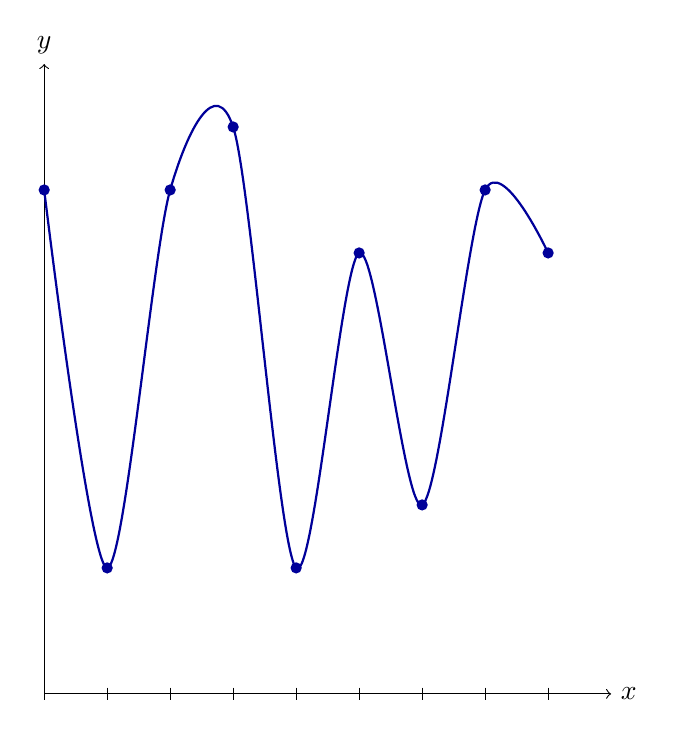
\begin{tikzpicture}[scale=0.8]
  \draw[->] (0,0) -- (9,0) node[right]{$x$};
  \draw[->] (0,0) -- (0,10) node[above]{$y$};
  \draw[thick,blue!60!black] plot[smooth,mark=*] coordinates {(0,8) (1,2) (2,8) (3,9) (4,2) (5,7) (6,3) (7,8) (8,7)};
  \foreach \i in {0,...,8} \draw (\i,0.1) -- (\i,-0.1);
\end{tikzpicture}
\caption{Synthetic series 7.2.}\label{fig:7-2}
\end{figure}
\section{Discussion}
\lipsum[27-32]
\begin{figure}[ht]
\centering
\begin{tikzpicture}[scale=0.8]
  \draw[->] (0,0) -- (8,0) node[right]{$x$};
  \draw[->] (0,0) -- (0,10) node[above]{$y$};
  \draw[thick,blue!60!black] plot[smooth,mark=*] coordinates {(0,3) (1,4) (2,5) (3,7) (4,4) (5,7) (6,3) (7,2)};
  \foreach \i in {0,...,7} \draw (\i,0.1) -- (\i,-0.1);
\end{tikzpicture}
\caption{Synthetic series 7.3.}\label{fig:7-3}
\end{figure}
\lipsum[33-36]
\lipsum[37-44] See Figure~\ref{fig:7-1} and Equation~\ref{eq:7}.
